\newpage
\subsection{Xây dựng hệ thống}

Với yêu cầu của bài toán, ta cần xây dựng hệ thống quản lý văn bằng cho các cơ sở giáo dục, và hệ thống tra cứu thông tin văn bằng cho phía doanh nghiệp (hoặc người có nhu cầu tra cứu).\\

\begin{figure}[ht]
    \centering
    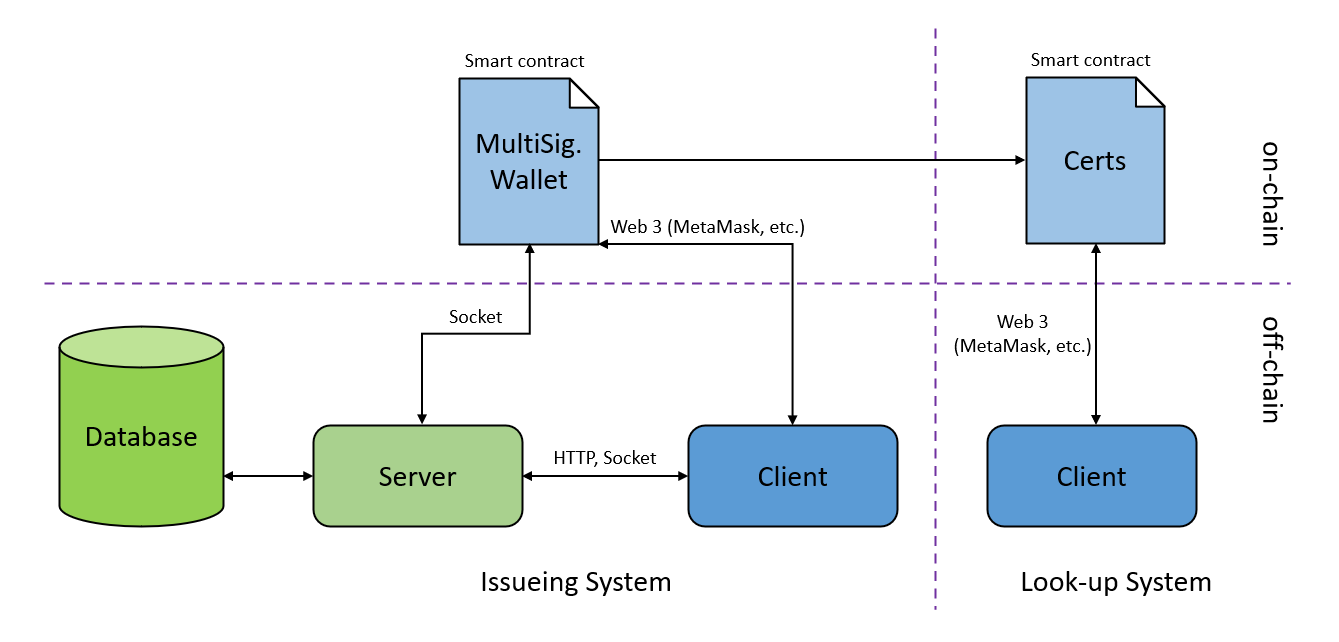
\includegraphics[width=400px]{images/system-overview.png}
    \caption{Sơ đồ tổng quan các hệ thống và mạng chuỗi khối}
    \label{images/system-overview}
\end{figure}

Những hệ thống này sẽ tương tác với các hợp đồng thông minh trên mạng chuỗi khối, bao gồm \textit{Kho văn bằng} (Certs) và \textit{Ví đa chữ ký} (MultiSig. Wallet). Trong bài báo cáo này, em xin phép tập trung trình bày về phần thiết kế các hợp đồng thông minh được triển khai cùng hệ thống.


\subsubsection{Kho văn bằng}
\textit{Kho văn bằng} (hay \textit{kho chứng chỉ}) là một hợp đồng thông minh nắm giữ thông tin các văn bằng được lưu trữ trên mạng chuỗi khối. Thông tin được tổ chức theo cấu trúc dạng cây, nắm giữ địa chỉ ví của các cơ sở giáo dục và danh sách các văn bằng cơ sở đó đã cấp phát.\\

Để lưu trữ văn bằng trên mạng chuỗi khối, các cơ sở giáo dục cần sử dụng một địa chỉ ví để tương tác với hợp đồng thông minh được triển khai trên mạng đó. Mỗi cơ sở phát hành văn bằng sẽ có một địa chỉ ví xác định, và trên cấu trúc cây được mô tả như trên, địa chỉ này sẽ được lưu trữ ở các \textit{nút bậc 1} (level-1 node), ký hiệu \texttt{School Address}; thông tin văn bằng được thể hiện qua các số hiệu tương ứng với các \textit{nút lá} (leaf) với ký hiệu \texttt{Certificate No.}.\\

\begin{figure}[!ht]
    \centering
    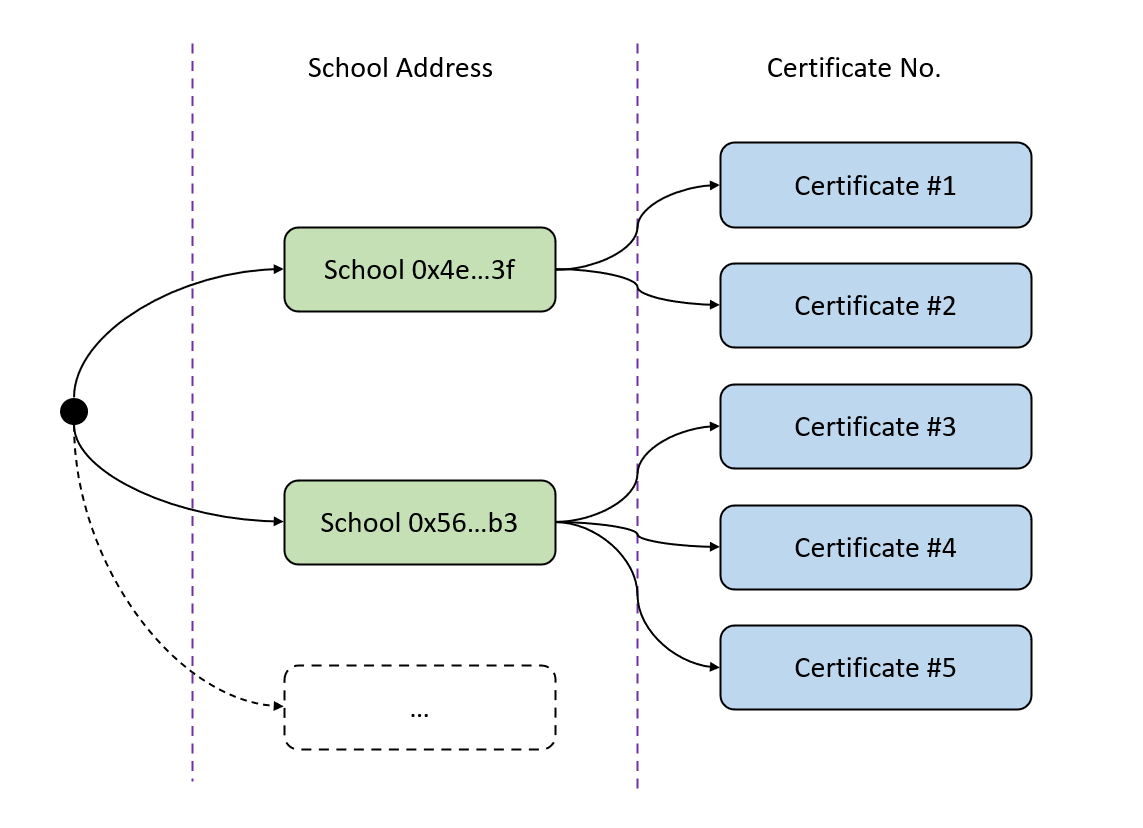
\includegraphics[width=400px]{images/certs-tree.png}
    \caption{Cấu trúc lưu trữ thông tin trong \textit{kho văn bằng}}
\end{figure}

\textit{Kho văn bằng} cung cấp một số chức năng liên quan đến lưu thông tin, tra cứu thông tin văn bằng, phụ lục văn bằng, thông tin của các cơ sở giáo dục, tổ chức cấp phát văn bằng, chứng chỉ. Tuy nhiên, trong phạm vi bài báo cáo này, ta quan tâm đến hai chức năng cơ bản:
\begin{itemize}
    \item Lưu thông tin văn bằng
    \item Xem thông tin văn bằng
\end{itemize}

Đối với việc \textit{lưu thông tin}, địa chỉ ví của cơ sở (hay người) gửi yêu cầu lưu thông tin văn bằng sẽ được lấy làm \texttt{School Address}, và thông tin được gửi khi tương tác với hợp đồng thông minh sẽ được lưu tương ứng với số hiệu \texttt{Certificate No.}. Như vậy, sẽ không có tình huống một cơ sở giáo dục phát hành văn bằng với địa chỉ của cơ sở khác, trường hợp nhầm lẫn do vô ý hoặc có chủ đích không thể xảy ra.\\

Để \textit{xem thông tin}, người tra cứu cần cung cấp địa chỉ ví của cơ sở phát hành văn bằng (\texttt{School Address}), và số hiệu văn bằng của cơ sở đó (\texttt{Certificate No.}).


\subsubsection{Ví đa chữ ký}
\textit{Ví đa chữ ký} là một hợp đồng thông minh với mục đích tăng tính bảo mật cho quá trình tương tác thay đổi thông tin văn bằng trên chuỗi khối.\\

Với việc "đẩy" thông tin văn bằng lên mạng chuỗi khối một cách thông thường, mỗi cơ sở giáo dục sử dụng địa chỉ ví của một cá nhân đại diện để tương tác, hoặc lựa chọn một địa chỉ ví và sử dụng chung cho cá nhân trong cơ sở. Điều này đảm bảo mỗi cơ sở cấp phát chứng chỉ có một địa chỉ \texttt{School Address} duy nhất. Tuy nhiên, khi nhiều cá nhân cùng dùng một địa chỉ ví, khả năng mất cắp tài sản liên kết với địa chỉ này càng lớn, đặc biệt khi nó còn được sử dụng trong các giao dịch khác có giá trị về tài chính (như địa chỉ sở hữu tiền mã hoá với giá trị cao trên các \textit{sàn giao dịch}\footnote{Exchange}, hay liên kết với các \textit{DApp} khác). Do đó, một cơ chế giúp giảm thiểu khả năng nhiều người cùng sở hữu một địa chỉ ví và có thể sử dụng địa chỉ ví để xác thực thông tin cơ sở cấp phát văn bằng là vô cùng cần thiết. \textit{Ví đa chữ ký} ra đời để giải quyết vấn đề này.\\

Không giống với các \textit{hệ thống xác thực đa chữ ký}\footnote{Multi-signature authentication system} khi ít nhiều phụ thuộc vào các cơ chế xác thực phức tạp, \textit{ví đa chữ ký} sử dụng các tính năng, lợi thế của hợp đồng thông minh và mạng chuỗi khối. Ở \textit{ví đa chữ ký}, mỗi hành động cần thực thi (ở đây là việc cấp phát văn bằng) yêu cầu một số lượng nhất định sự đồng ý từ cá nhân. Địa chỉ ví của các cá nhân này đã được thêm vào danh sách "thành viên" ngay từ khi hợp đồng thông minh này được triển khai, và họ được coi như các "cổ đông" của "doanh nghiệp" cấp phát văn bằng khi có "tiếng nói" trong các "hoạt động" ở đây. Mỗi cơ sở cấp phát văn bằng sử dụng một \textit{ví đa chữ ký} duy nhất, và địa chỉ của hợp đồng thông minh này đại diện cho địa chỉ ví của cả cơ sở đó. Các văn bằng cần được đẩy lên \textit{kho văn bằng} sẽ được một cá nhân trong cơ sở gửi lên "ví" này. Các thành viên khác trong cơ sở có thể xem thông tin các văn bằng được gửi lên, và đưa ra biểu quyết "đồng ý" hay "không đồng ý" trên hợp đồng thông minh. Khi số lượng sự đồng ý đạt ngưỡng nhất định (được thiết lập từ đầu), các văn bằng đó được đẩy lên "kho", và thông tin được lưu trữ trên mạng chuỗi khối.\\

\begin{figure}[!ht]
    \centering
    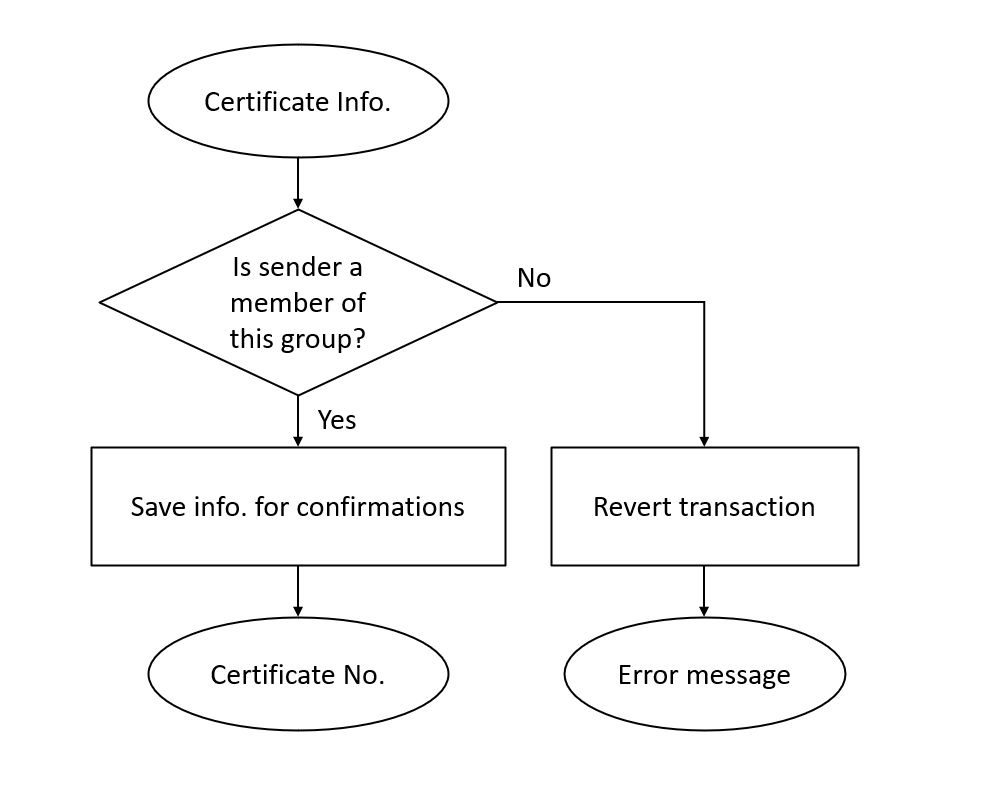
\includegraphics[width=300px]{images/multisig-add-cert.png}
    \caption{Tạo yêu cầu cấp phát văn bằng lên \textit{ví đa chữ ký}}
\end{figure}

\begin{figure}[!ht]
    \centering
    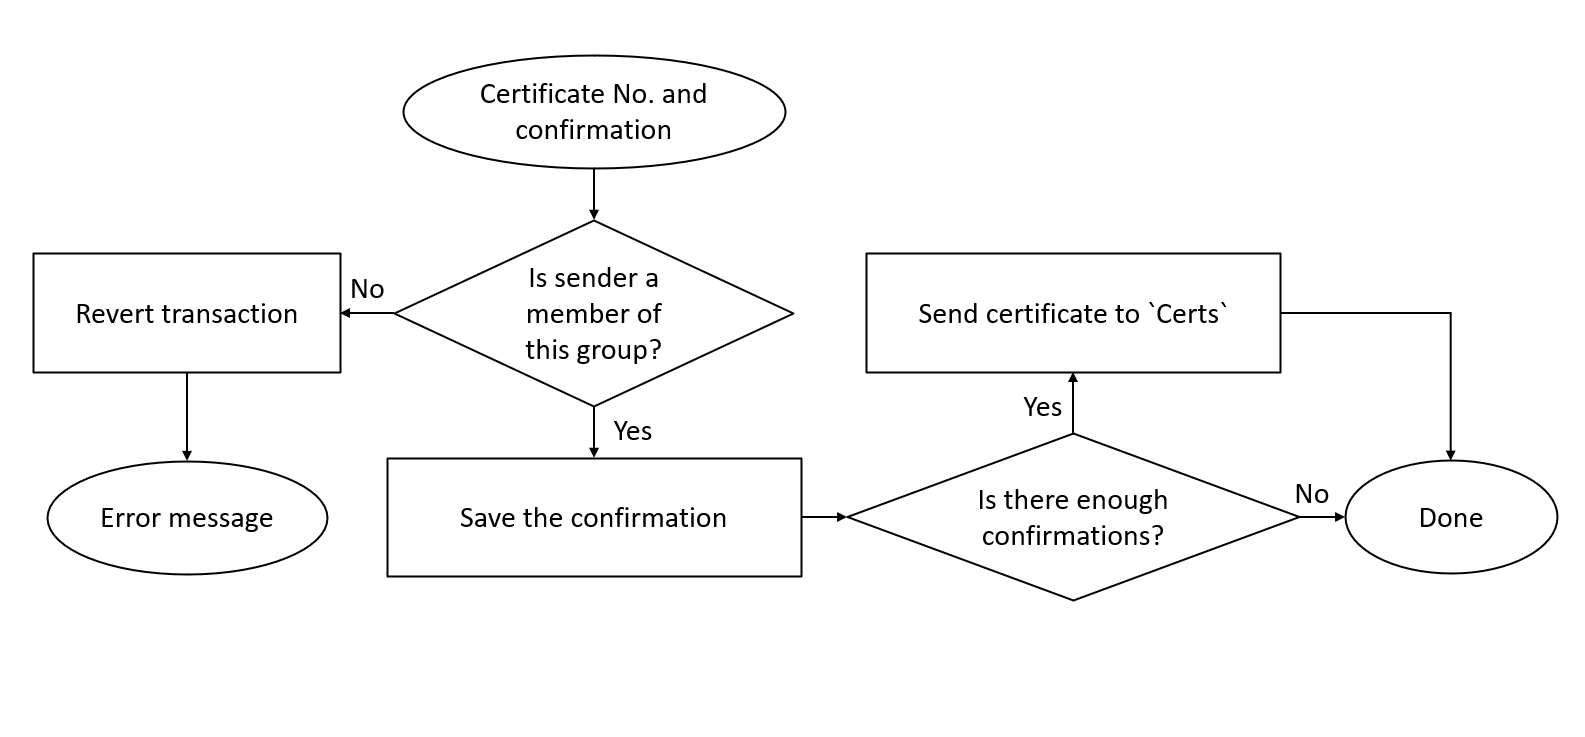
\includegraphics[width=400px]{images/multisig-confirm-cert.png}
    \caption{Đưa ra biểu quyết để đưa văn bằng trên "ví" lên "kho"}
\end{figure}


\subsubsection{Các yêu cầu liên quan}
Với \textit{hệ thống tra cứu}, không có có quá nhiều yêu cầu cần thực hiện. Hiện nay, các tiện ích, phần mềm được tạo ra, đáp ứng nhu cầu kết nối đến mạng chuỗi khối, trong số đó có thể kể đến \href{https://github.com/ChainSafe/web3.js}{\textit{Web3.js}}. \textit{Web3.js} là một dự án mã nguồn mở của \textit{ChainSafe}, được viết chủ yếu bởi ngôn ngữ lập trình \textit{JavaScript}, cung cấp các công cụ giúp người dùng tương tác với mạng Ethereum và các hợp đồng thông minh trên mạng này. \textit{Web3.js} có thể được tích hợp cho các \textit{DApp} dạng \textit{web}\footnote{Website} (webapp). Việc tra cứu thông tin văn bằng trở nên đơn giản và hết sức thân thiện, khi người dùng có thể trực tiếp thao tác qua giao diện trên trình duyệt.\\

Đối với \textit{hệ thống quản lý}, yêu cầu quan trọng nhất của hệ thống là ghi lại thông tin các văn bằng được tạo ra. Các văn bằng này sau khi được cấp phát cần được cập nhật trạng thái để tránh việc đẩy nhiều lần lên chuỗi khối. Mặc dù việc gửi một văn bằng nhiều lần lên chuỗi khối không gây ảnh hưởng xấu gì về mặt thông tin do các thiết kế các hợp đồng thông minh không cho phép hai văn bằng cùng \texttt{School Address} và \texttt{Certificate No.} cùng tồn tại; tuy nhiên, mỗi khi tương tác với hợp đồng thông minh, chi phí giao dịch sẽ phát sinh. Như đã trình bày ở \textit{Hình \ref{images/system-overview}}, phía \textit{máy chủ} (server) sẽ lắng nghe các \textit{sự kiện} (event) khi trạng thái của hợp đồng thông minh thay đổi, nhanh chóng cập nhật thông tin tương ứng trong \textit{cơ sở dữ liệu}, và thông báo lên giao diện người dùng. Ở hệ thống này, để tương tác được với hợp đồng thông minh, các thành viên trong cơ sở cấp phát văn bằng cần sử dụng thêm một \textit{ví mã hoá}\footnote{Crypto wallet} lưu trữ các địa chỉ ví của họ. Một số ví mã hoá phổ biến có thể kể đến như \href{https://metamask.io/}{\textit{MetaMask}}, \textit{Coinbase}.\\

Việc thiết kế cơ sở dữ liệu cũng cần đảm bảo đáp ứng các yêu cầu của một hệ thống tương tác với chuỗi khối. Đối với những thực thể cần được lưu trữ trên mạng chuỗi khối, ta cần thêm một số thuộc tính định danh trên chuỗi khối. Cụ thể, trong thiết kế cơ sở dữ liệu, bảng \texttt{certificates} lưu trữ thông tin cho các văn bằng mà cơ sở giáo dục cấp phát. Ngoài các trường cơ bản - như \textit{số hiệu văn bằng} (cột \texttt{reg\_no} trong bảng), \textit{tên người được cấp phát văn bằng} (\texttt{conferred\_on}), \textit{chuyên ngành} (\texttt{major\_in}), \textit{tên loại văn bằng} (\texttt{degree\_of}), \textit{đánh giá văn bằng} hay \textit{xếp loại} (\texttt{degree\_classification}), \textit{hình thức đào tạo} (\texttt{mode\_of\_study}), \textit{nơi cấp} (\texttt{created\_in}) và \textit{ngày cấp} (\texttt{created\_at}) - trường \textit{định danh trên chuỗi} (tương ứng với cột \texttt{on\_chain\_id} trong bảng) giúp lưu trữ liên kết giữa dữ liệu trong hệ thống quản lý và mạng chuỗi khối. Để giảm chi phí giao dịch khi tương tác với hợp đồng thông minh, các văn bằng được gom lại thành những \textit{lô} (batch), và được đẩy lên chuỗi khối đồng thời. Chính vì vậy, bảng \texttt{certificates} cần thêm một cột lưu thông tin định danh cho các lô được cấp phát, ký hiệu là \texttt{batch\_reg\_no}. Thông tin các lô văn bằng này được thể hiện tương ứng trong bảng \texttt{batches}, với các trường thông tin liên quan tới \textit{định danh} \texttt{reg\_no}, \textit{người tạo} (\texttt{creator\_id}), và tất nhiên là cả \textit{định danh trên chuỗi} (\texttt{on\_chain\_id}).\\

\begin{figure}[!ht]
    \centering
    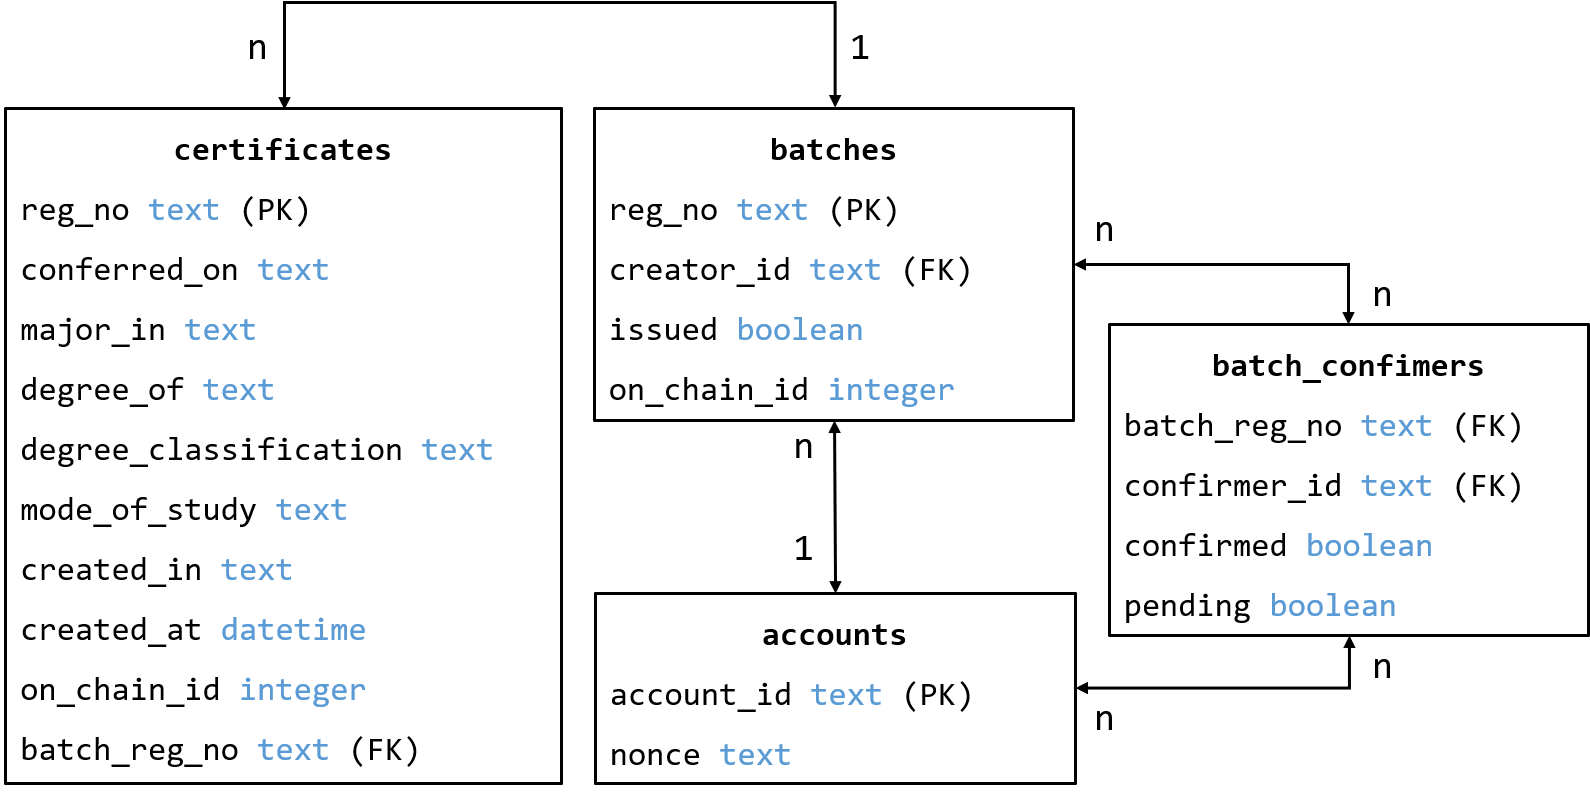
\includegraphics[width=400px]{images/database.png}
    \caption{Biểu đồ cơ sở dữ liệu cho hệ thống quản lý.}
\end{figure}

Với các thành viên tham gia cấp phát văn bằng, thông tin được lưu trong bảng \texttt{accounts}. Để truy cập vào hệ thống quản lý này, như thông thường, các thành viên cần xác thực tài khoản. Nhằm tận dụng các tính năng bảo mật của \textit{mã hoá bất đối xứng}\footnote{Asymmetric cryptography} (cụ thể là \textit{chữ ký số}\footnote{Digital signature}), em xin mang đến một cách xác thực nhanh gọn và an toàn qua ví MetaMask, tạm gọi là "xác thực một nút". Với cách xác thực này, mỗi khi một thành viên muốn truy cập vào hệ thống, một thông điệp ngẫu nhiên sẽ được gửi tới và họ cần ký thông điệp này và gửi lại cho máy chủ hệ thống. Việc "ký" thông điệp hoàn toàn được hỗ trợ bởi ví MetaMask với chỉ một thao tác bấm nút đơn giản. Đồng thời, tính hợp lệ của chữ ký cũng được kiểm tra một cách nhanh chóng dựa trên các trường thông tin như địa chỉ ví và thông điệp. Sau đó, một \textit{mã xác thực có thời hạn}\footnote{Expirable token} được gửi lại cho phía thành viên, giúp họ tương tác với hệ thống trong một khoảng thời gian nhất định mà không cần phải đăng nhập lại. Với cách xác thực này, các thành viên tham gia cấp phát văn bằng không cần ghi nhớ mật khẩu để đăng nhập, mức độ bảo mật cho hệ thống cũng được đảm bảo. Và quay trở lại bảng \texttt{accounts}, định danh cho thành viên trong hệ thống sẽ tương ứng với \textit{địa chỉ ví}, được lưu trong cột \texttt{account\_id}, và thông điệp (message) dùng được ghi lại tương ứng với cột \texttt{nonce} (cách đặt tên dựa theo BitCoin) trong bảng.\\

\clearpage
\begin{figure}[ht]
    \centering
    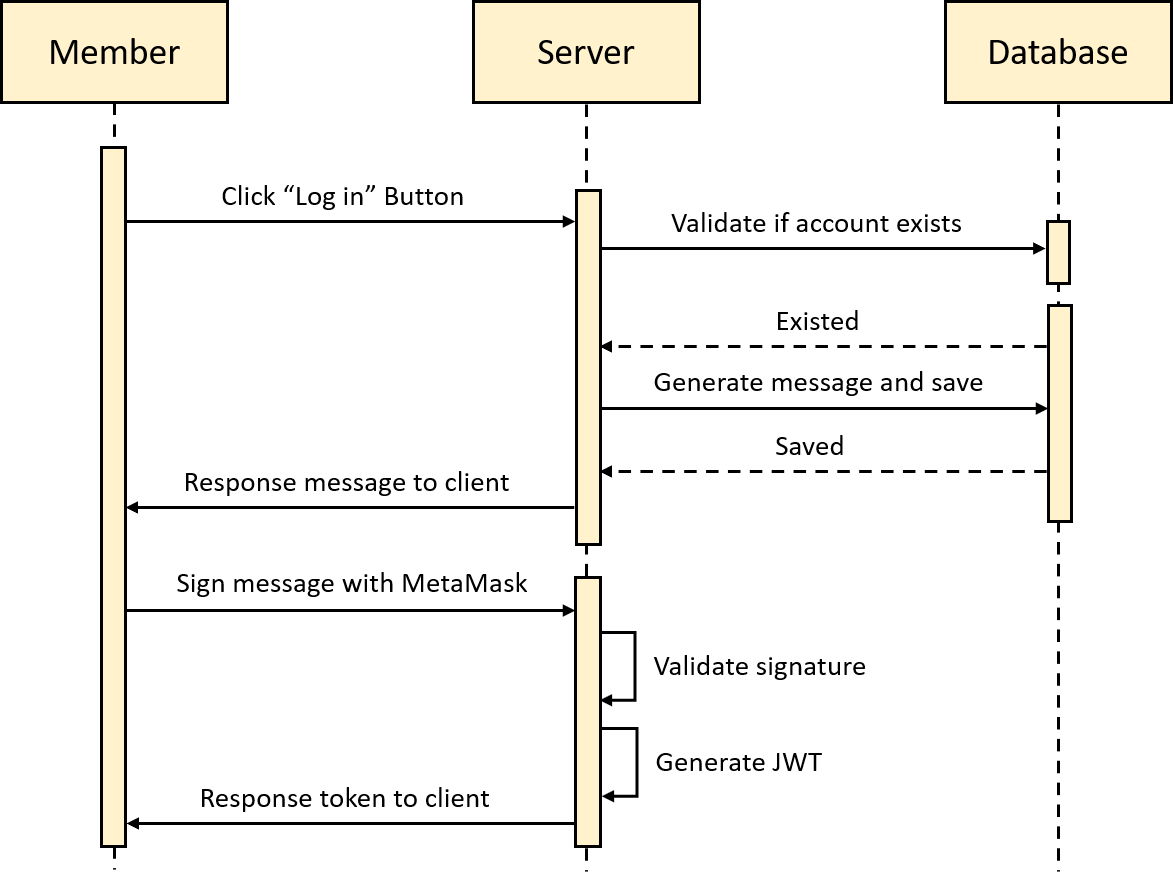
\includegraphics[width=400px]{images/login-flow.png}
    \caption{Biểu đồ trình tự đăng nhập với "xác thực một nút".}
\end{figure}

Với việc sử dụng đa xác thực bằng ví MetaMask, mỗi khi một lô văn bằng cần được đẩy lên mạng chuỗi khối, mỗi thành viên cần biểu quyết đồng ý hoặc từ chối. Thông tin về các biểu quyết này được lưu trong bảng \texttt{batch\_confirmers}, với hai \textit{khoá ngoại lai}\footnote{Foreign key - FK} (FK) tương ứng với các khoá chính của bảng \texttt{accounts} và bảng \texttt{batches}.\\

